\documentclass[10pt]{article}
\usepackage[margin=0.65in]{geometry}
\usepackage{amsmath,amssymb,hyperref,tikz}
\usetikzlibrary{positioning,arrows.meta}
\title{Representation joins: paper and implementation boundary}
\author{Research implementation report}
\date{21 October 2026}
\begin{document}
\begin{center}\Large Representation joins: paper and implementation boundary\\[4pt]
\normalsize Research implementation report --- 21 October 2026\end{center}
\noindent\textbf{Status.} Bounded native reference implementation, with an index-calculus
relation adapter. No timing or asymptotic improvement is claimed. The full
fast backend and production collector integration remain open.

\paragraph{The paper.} Delaplace, Fouque, Kirchner and May,
\emph{Solving ECDLP over $\mathbb F_{p^\ell}$ with Pre-computation via
Representation Technique}, 2020, \url{https://inria.hal.science/hal-02427655v1}.
For $Q=kP$, represent $k=k_{11}+k_{12}+k_{21}+k_{22}\pmod r$ in many ways.
Join two pairs of lists, retain intermediate points with $x\in\mathbb F_p$,
and match full points. The match determines a scalar candidate, checked by
replaying $kP=Q$. The paper uses polynomial multipoint evaluation to avoid
testing every pair. Its quadratic-field setup is approximately $p^{6/5}$,
online work and memory $p^{4/5}$, under its heuristics and suppressed overheads.
This does not improve the prior Bernstein--Lange precomputation tradeoff.

\begin{center}
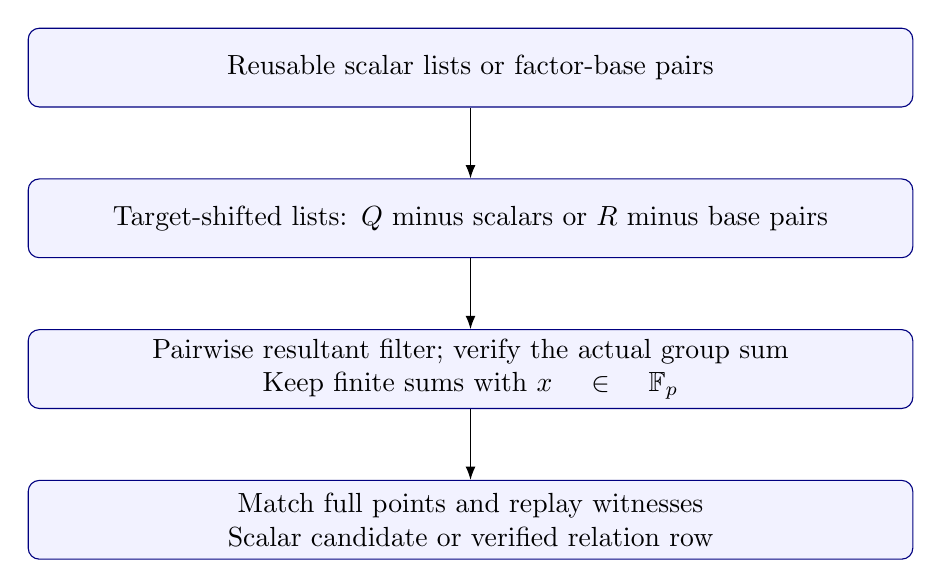
\begin{tikzpicture}[node distance=9mm,box/.style={draw=blue!50!black,fill=blue!5,rounded corners,align=center,text width=11cm,minimum height=10mm},>=Latex]
\node[box](a){Reusable scalar lists or factor-base pairs};
\node[box,below=of a](b){Target-shifted lists: $Q$ minus scalars or $R$ minus base pairs};
\node[box,below=of b](c){Pairwise resultant filter; verify the actual group sum\\Keep finite sums with $x\in\mathbb F_p$};
\node[box,below=of c](d){Match full points and replay witnesses\\Scalar candidate or verified relation row};
\draw[->](a)--(b);\draw[->](b)--(c);\draw[->](c)--(d);
\end{tikzpicture}
\end{center}
\noindent Diagram: implemented reference stages, not measured costs. The SVG
companion shows the left and right inputs separately.

\paragraph{Connection to index calculus.} The adapter emits witnesses for
$aP+bQ=B_i+B_j+B_k+B_l$ with the filtered intermediate. These give rows
$a+bk=\sum_j c_j\log_P(B_j)\pmod r$ after the caller validates a common
prime-order subgroup. This is a restricted decomposition oracle; its missing
unfiltered witnesses must not be counted as complete PDP coverage.

\paragraph{What is implemented.} C++17 quadratic-field arithmetic, validated
curves, direct and resultant-filter joins, reusable four-list setup, target
matching, and coefficient rows retaining witness multiplicities. The
resultant is a necessary test, followed by exact addition. Zero determinants
can be false positives; infinity and doubling take exact paths. Complexity
is still pairwise; bounded membership enumeration costs $O(r)$.

\paragraph{Checks and limitations.} Three fixtures over $p=5,7,11$ compare
complete join outputs with direct addition; positive subgroups have orders
7 and 137, with all 144 targets checked. The $p=7$ order-3 subgroup is a
zero-yield negative control. Four-index enumeration checks the PDP witness
sets; it shares arithmetic with the candidate. See
\texttt{records/final-check.txt} and \texttt{records/sanitizer.txt} for
exact results. Earlier fixture failures are retained. These are unit tests,
not independent-host replay or performance experiments.

\paragraph{Open work.} Symbolic product polynomials, Kedlaya--Umans evaluation,
optimized scalar partitions, general extension fields, production collector
wiring, rank/LA/descent, and matched end-to-end costs. Prime fields have no
proper subfield for this filter. Cargo and Conductor were unavailable locally.
No leaderboard, benchmark index, or curve/isogeny graph is promoted.
\end{document}
